\documentclass{article}

\usepackage{amsmath, amsfonts, amsthm, amssymb} 
\usepackage{listings}
\usepackage{graphicx}
\usepackage{float}
\usepackage{subfigure}
\usepackage{geometry}
\usepackage{hyperref}
\usepackage[parfill]{parskip} % no newline indent
\usepackage{enumitem} % enumerate / ordered list
\usepackage{booktabs} % three-line table
\usepackage{array}   % for \newcolumntype macro
\usepackage{listings} % MATLAB code block
\newcolumntype{C}{>{$}c<{$}} % math-mode version of "l" column type

\theoremstyle{definition} % difinition
\newtheorem{definition}{Definition}[section]
\newtheorem{theorem}{Theorem}[section]
\newtheorem{remark}{Remark}[section]

\newcommand{\dd}{\mathrm{d}}
\newcommand{\RR}{\mathbb{R}}
\newcommand{\NN}{\mathbb{N}}
\newcommand{\ZZ}{\mathbb{Z}}
\newcommand{\CC}{\mathbb{C}}
\newcommand{\PP}{\mathbb{P}}


\lstset{
  language=Matlab,  %代码语言使用的是matlab
  frame=shadowbox, %把代码用带有阴影的框圈起来
  numbers=left, % 显示行号
  breaklines=true
}

\geometry{
	paper=a4paper, 
	top=2.5cm,
	bottom=2.5cm, 
	left=2.5cm, 
	right=3cm,
	headsep=0.75cm, 
}
\title{ROB 501 HW6}
\author{Yulun Zhuang \\ \href{mailto:yulunz@umich.edu}{yulunz@umich.edu}}
\date{\today}

\begin{document}

\maketitle

\section{}
\begin{align*}
    y_1 &=\left[\begin{array}{c}
    -2 \\
    1 \\
    1
    \end{array}\right], y_2=\left[\begin{array}{l}
    0 \\
    4 \\
    1
    \end{array}\right], y_3=\left[\begin{array}{c}
    4 \\
    -4 \\
    6
    \end{array}\right] \\
    v_1 &=\left[\begin{array}{c}
    -2 \\
    1 \\
    1
    \end{array}\right]\\
    \left\|v_1\right\| &= \sqrt{6} \\
    v_2 &=y_2-\frac{\left\langle v_1, y_2\right\rangle}{\left\|v_1\right\|^2} \cdot v_1 \\
    &=\left[\begin{array}{c}
    0 \\
    4 \\
    -1
    \end{array}\right]-\frac{3}{6} \cdot\left[\begin{array}{r}
    -2 \\
    1 \\
    1
    \end{array}\right] \\
    &=\left[\begin{array}{c}
    1 \\
    \frac{7}{2} \\
    -\frac{3}{2}
    \end{array}\right] \\
    \left\|v_2\right\| &=\sqrt{\frac{31}{2}}\\
    v_3 &=y_3-\frac{\left\langle v_1, y_3\right\rangle}{\left\|v_1\right\|^2} v_1-\frac{\left\langle v_2, y_3\right\rangle}{\left\|v_2\right\|^2} v_2 \\
    &=\left[\begin{array}{c}
    4 \\
    -4 \\
    6
    \end{array}\right]+\left[\begin{array}{c}
    -2 \\
    1 \\
    1
    \end{array}\right]+\frac{19}{31}\left[\begin{array}{c}
    2 \\
    7 \\
    -3
    \end{array}\right] \\
    &=\left[\begin{array}{c}
    100/31 \\ 40/31 \\ 160/31
    \end{array}\right]
\end{align*}


\section{}
\subsection{}
\begin{figure}[H]
    \centering
        \textsf{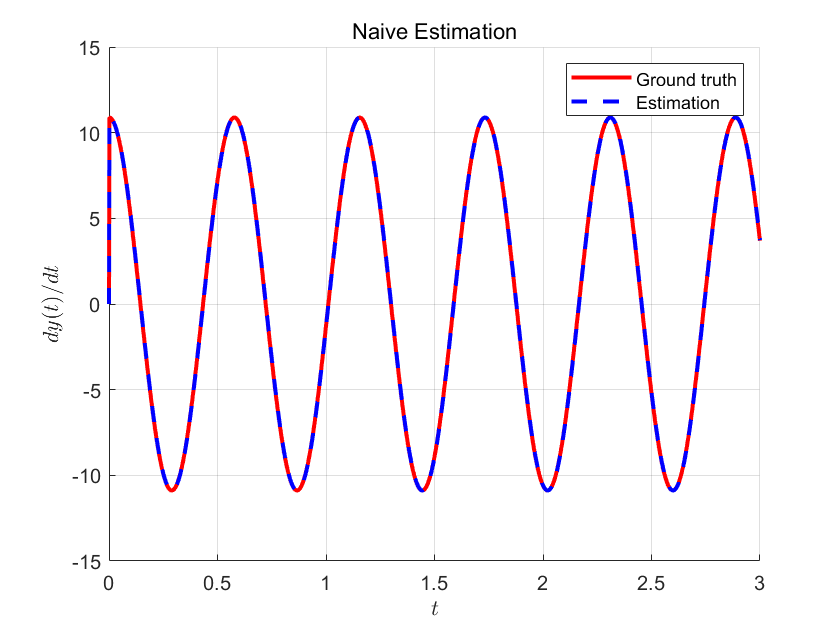
\includegraphics[width=0.6\columnwidth]{hw6-prob2-fig1.png}}
        \caption{Naive estimation of the derivative of $y(t)$}
        \label{fig: 2-1}
\end{figure}


\subsection{}
The function I used is $\hat{y}(t) = c_0 + c_1 t + c_2 t^2 + c_3 t^3 + c_4 t^4 + c_5 t^5$. And the window size is $7$.
\begin{figure}[H]
    \centering
        \textsf{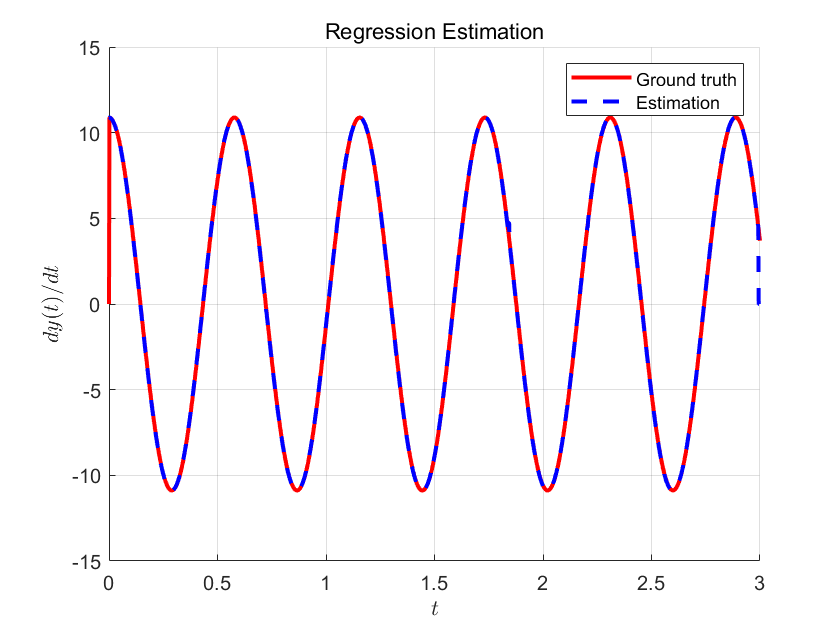
\includegraphics[width=0.6\columnwidth]{hw6-prob2-fig2.png}}
        \caption{Regression estimation of the derivative of $y(t)$}
        \label{fig: 2-2}
\end{figure}


\section{}

\subsection{}

The function I used is $\hat{y}(t) = c_0 + c_1 t + c_2 t^2 + c_3 t^3 + c_4 t^4 + c_5 t^5$. And the window size is $14$.

\begin{figure}[H]
    \centering
        \textsf{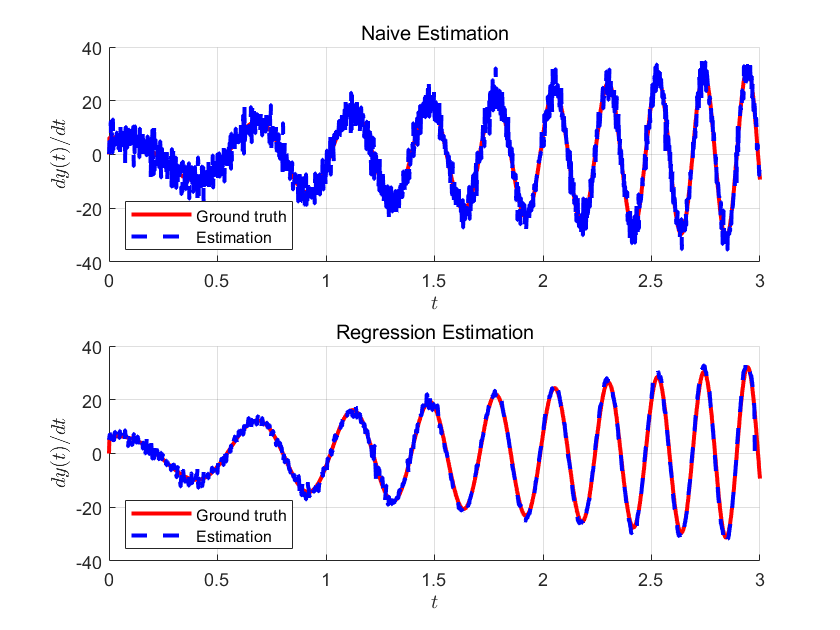
\includegraphics[width=0.6\columnwidth]{hw6-prob3-fig1.png}}
        \caption{Estimations of the derivative of $y(t)$}
        \label{fig: 3-1}
\end{figure}

\subsection{}
The Root mean Square Error(RMSE) for the naive estimation is 3.5854, and the RMSE for the regression estimation is 1.3508.

\section{}

Given $\mathcal X = \RR^{2,2}$, $<A, B> = tr(A^TB)$ and $M = span\left\{ y_1, y_2\right\}$

$$
y_1 = 
\begin{bmatrix}
    1 & 0 \\ 2 & 0
\end{bmatrix}, \ 
y_2 = 
\begin{bmatrix}
    1 & 1 \\ 1 & 1
\end{bmatrix}
$$

Solve $\hat x = arg\min_{y\in M} \|x-y\|$ when 
$
x = 
\begin{bmatrix}
    0 & -1 \\ 2 & 0
\end{bmatrix}
$

Apply the Normal Equations,

\begin{align*}
    G^{\top} \alpha&=\beta\\
    G&=\left[\begin{array}{ll}
    \left\langle y^{1}, y^{1}\right\rangle, & \left\langle y^{1}, y^2\right\rangle \\
    \left\langle y^2, y^{1}\right\rangle, & \left\langle y^2, y^2\right\rangle
    \end{array}\right]=\left[\begin{array}{ll}
    5 & 3 \\
    3 & 4
    \end{array}\right]\\
    \beta&=\left[\begin{array}{c}
    \left\langle x, y^{1}\right\rangle \\
    \left\langle x, y^2\right\rangle
    \end{array}\right]=\left[\begin{array}{l}
    4 \\
    1
    \end{array}\right]\\
    \Rightarrow \ \alpha&=\left[\begin{array}{cc}
    \left\langle y^{1}, y^{1}\right\rangle & \left\langle y^2, y^{1}\right\rangle \\
    \left\langle y^{1}, y^2\right\rangle & \left\langle y^2, y^2\right\rangle
    \end{array}\right]^{-1}\left[\begin{array}{c}
    \left\langle x, y^{1}\right\rangle \\
    \left\langle x, y^2\right\rangle
    \end{array}\right]\\
    &=\frac{1}{11}\left[\begin{array}{cc}
    4 & -3 \\
    -3 & 5
    \end{array}\right]\left[\begin{array}{l}
    4 \\
    2
    \end{array}\right]\\
    &=
    \begin{bmatrix}
        13/11 \\ -7/11
    \end{bmatrix}\\
    \Rightarrow \ \hat x &= \alpha_1 y^{1}+\alpha_2 y^2 = 
    \begin{bmatrix}
        6/11 & -7/11 \\ 19/11 & -7/11
    \end{bmatrix}
\end{align*}


\section{}
Given $(x, \mathbb{R},\|\cdot\|)$ is strictly normed. $M$ is a subspace of $x$, Show that if exists $m^* \in M$,
$$
\text { s.t. }\|x-m^*\|=d(x, M):=\inf _{\substack{y \in M}}\|x-y\|
$$
then $m$ is unique.

\begin{proof}
    Suppose $m_1, m_2 \in M$ satisfy $\|x-m_i\| = d(x, M), i=1,2$.\\
    Let $\gamma = d(x, M)$, and note that $(m_1+m_2)/2 \in M$.
    \begin{align*}
        \gamma &=\inf _{y \in M}\|x-y\| \\
        &\leq\left\|x-\frac{m_1+m_2}{2}\right\| \\
        &=\left\|\frac{x-m_1}{2}+\frac{x-m_2}{2}\right\| \\
        &\leq \frac{1}{2}\left\|x-m_1\right\|+\frac{1}{2}\left\|x-m_2\right\| \\
        &=\frac{\gamma}{2}+\frac{\gamma}{2}=\gamma   
    \end{align*}
    implies $\left\|\frac{x-m_1}{2}+\frac{x-m_2}{2}\right\| = \frac{1}{2}\left\|x-m_1\right\|+\frac{1}{2}\left\|x-m_2\right\|$\\
    Since the norm space is strictly normed, 
    $$
    \frac{x-m_1}{2}=\alpha \frac{x-m_2}{2} \Rightarrow\left\|\frac{x-m_1}{2}\right\|=\alpha \left\|\frac{x-m_2}{2}\right\|.
    $$
    Hence $\alpha=1$ and $\frac{x-m_1}{2}=\frac{x-m_2}{2} \Rightarrow m_1=m_2$
\end{proof}

\section{}
Given $ x\in \RR^2, \ x = [x_1, x_2]^T$.

\begin{enumerate}[label=(\alph*)]
    \item $\|x\|_1=\left|x_1\right|+\left|x_2\right|$
        \begin{align*}
            \text{Let } x=\left[\begin{array}{l}
            0 \\
            1
            \end{array}\right],\ y=\left[\begin{array}{l}
            1 \\
            0
            \end{array}\right] \\
            \|x+y\|_1=2 \\
            \|x\|_1+\|y\|_1=1+1=2
        \end{align*}
        Since $\|x+y\|=\|x\|+\|y\|$, but $x$ and $y$ is not related by a non-negative factor.
    \item $\|x\|_{\infty}=\max \left\{\left|x_1\right|,\left|x_2\right|\right\}$
        \begin{align*}
            \text{Let } x=\left[\begin{array}{l}0 \\ 0\end{array}\right],\ y=\left[\begin{array}{l}1 \\ 0\end{array}\right]\\
            \|x+y\|_{\infty}=1\\
            \|x\|_{\infty}+\|y\|_{\infty}=0+1=1\\
        \end{align*}
        Since $\|x+y\|=\|x\|+\|y\|$, but $x$ and $y$ is not related by a non-negative factor.
\end{enumerate}


\section{}
\begin{lstlisting}
function result = MatrixInversionLemma(A_inv, B, C, D)
    result = A_inv - A_inv * B * inv(inv(C) + D * A_inv * B) * D * A_inv;
end
\end{lstlisting}



\section{}
Given 
$$
\begin{aligned}
&x=\{f \mid f: \mathbb{R} \rightarrow \mathbb{R}\}, F=\mathbb{R} \\
&\text { Define }\langle f, g\rangle=\int_{-1}^1 f(t) g(t) d t \\
&M=\operatorname{span}\left\{1, t, \frac{1}{2}\left(3 t^2-1\right)\right\}, \quad x=e^t
\end{aligned}
$$
Find $\hat{x}=\arg \min_{y\in M} \|x-y\|$

\begin{align*}
    G^{T} \alpha&=\beta \text { where } G_{i j}=\left\langle y^i, y^j\right\rangle, \beta_i =\left\langle x, y^i\right\rangle\\
    G&=\left[\begin{array}{ccc}
    2 & 0 & 0 \\
    0 & \frac{2}{3} & 0 \\
    0 & 0 & \frac{2}{5}
    \end{array}\right]\\
    \beta&=\left[\begin{array}{c}
    e-e^{-1} \\
    2 e^{-1} \\
    e-7 e^{-1}
    \end{array}\right]\\
    \alpha&=G^{-T} \beta\\
    &=\left[\begin{array}{ccc}
    \frac{1}{2} & 0 & 2 \\
    0 & \frac{3}{2} & 0 \\
    0 & 0 & \frac{5}{2}
    \end{array}\right]\left[\begin{array}{c}
    e-e^{-1} \\
    2 e^{-1} \\
    e-7 e^{-1}
    \end{array}\right]\\
    &=\left[\begin{array}{c}
    \frac{1}{2}\left(e-e^{-1}\right) \\
    3 e^{-1} \\
    \frac{5}{2}\left(e-7 e^{-1}\right)
    \end{array}\right]\\
    \hat{x}&= \alpha_1 y^1 + \alpha_2 y^2 +\alpha_3 y^3\\
    &=\frac{1}{2}\left(e-e^{-1}\right)+3 e^{-1} t+\frac{5}{4}\left(e-7 e^{-1}\right)\left(3 t^2-1\right)
\end{align*}

\textbf{Discussion}:

In this problem's setup, we use orthogonal basis to compute the normal equations, while in recitation, we use naive polynomial basis $\{ t, t^2, t^3\}$. Note that when using orthogonal basis, the $G$ matrix is diagonal, which is easier to compute its inverse and gives reliable results comparing with naive polynomial basis.



\end{document}